\scanpage{9}
\mspage{7}

\noindent
\begin{minipage}{.06\linewidth}
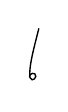
\begin{tikzpicture}[x=1em,y=1em]
\draw[line width=.5pt] (.5,2.1) .. controls (.35,1.5) and (.12,.7) .. (.18,.32)
 .. controls (.25,.12) and (.48,.35) .. (.35,.46)
 .. controls (.23,.52) and (.12,.38) .. (.18,.32);
\end{tikzpicture}
\end{minipage}
\begin{minipage}{.9\linewidth}
\begin{tabular}{|p{.94\linewidth}|}
\handwritten{Attention : la catégorie $\underline{\mathrm{Hom}}_{\mathrm{gr-b}}$, qui s'identifie à la catégorie définie
par un $\unsure{R|\mathbb{R}}\mathrm{Hom}_{\mathbb{Z}}(C_{\unsure{x|\bullet}}, C'_{\unsure{x|\bullet}})$; ce point devant être élucidé !}\\
\hline
\end{tabular}
\end{minipage}

de même les (Cat)-groupes(ou groupes à valeurs dans (Cat)) comme étant
les groupes semisimpliciaux qui ``sont''des catégories i.c. qui \deleted{se défini\unsure{s|d}}
\deleted{sent} sat\unsure{\deleted{s}i\deleted{i}s|\deleted{i}s\deleted{s}i}font la condition d'exactitude familière, permettant d'en déte
miner tous les composants à l'aide de $C_{o\deleted{a}}$ et $C_1$ . Appliquant le tapis de
Dold, dans le cas commutatif, on trouve que les (Cat)-groupes abéliens
forment une catégorie équivalente à celle des complexes de chaines de
groupes abéliens qui sont de longueur 1:
\[ 0 \leftarrow C_o \leftharpoonup C_1 \leftarrow 0 \quad . \]
Quand on explicite la (Cat)-groupe abélien associé à un tel complexe de
chaines, on trouve ``ma'' construction chérie da la ``catégorie de Picard''
associée au complexe: objets ceux de $C_o$ , flêches de x dans y les z dans
tels que $dz = y-x$ . On trouve donc à isomorphisme ppès tous les group\unsure{e}
abéliens de (Cat) ainsi. Un complément important est que toute catégori
\margin{\handwritten{\deleted{\unsure{Objection déjà}, mais cela contredit les \unsure{résultats} de \illegible{2 lignes}}}}
de Picard \deleted{\inserted{(resp. et} commutative)}est équivalente (au sens technique qu'on ne précis
pas ici) à \deleted{la catégorie} un vrai (Cat)-groupe \deleted{\inserted{(resp. (Cat)-groupe} commutatif)}\begin{tikzpicture}[x=1cm,y=1cm,baseline=0pt]\draw[line width=.45pt] (0,.7)--(.01,.5);\draw[line width=.45pt] (.03,.43)..controls(.1,.29)and(.3,.29)..(.5,.32);\draw[line width=.45pt] (.75,.2)..controls(.63,.02)and(.59,-.16)..(.61,-.35);\end{tikzpicture} .
\inserted{\handwritten{Quand on
\unsure{identifie|simplifie} mod ``\unsure{Gros|Grab}'' équivalence, cela correspond à travailler dans la catégorie \uline{déri\unsure{v}}
des complexes, seuls invariants \unsure{étant|sont} $\pi_o, \pi_1$)}}
\margin{\handwritten{\unsure{Mais} \unsure{si on part} d'une ``cat. de Picard \unsure{commut.}'' elle \unsure{ne se réalise} que par un $(\mathrm{Cat})$-g. \uline{\uline{\unsure{non}}} \uline{\unsure{comm.}}}}
On notera qu'on a une \deleted{\unsure{l|t}\illegible{5}} classification beaucoup plus restrein
que pour les H-espaces (resp. les H-espaces homotopiquement comm.) mod
équivalence d'homotopie, de façon précise entre les groupes resp. les gr
oupes abéliens de la catégorie homotopique. La raison en est qu\inserted{\handwritten{'}}on est beau
coup plus restrictif dans le contexte catégorique pour le sens d\unsure{a|e} l'asso\unsure{c}
tivité (resp. et de la commutativité), puisqu'on ne demande pas seulemen\unsure{t}
l'existence d'isomorphismes d'associ\unsure{\deleted{t}a|\deleted{a}t}itivité\deleted{\unsure{,}} (qui suffirait pour avoir \unsure{u}
groupe dans \begin{tabular}[b]{@{}l@{}}\inserted{la catégorie homotopique}\\[-.6ex]\begin{tikzpicture}[x=1cm,y=.7cm,baseline=0pt]\draw[line width=.45pt] (0,.8)..controls(-.1,.55)and(-.08,.16)..(.18,.14)..controls(.4,.13)and(.57,.23)..(.8,.18)--(1.7,.16)..controls(1.8,.15)and(1.87,.1)..(1.95,.09);\draw[line width=.45pt] (2.02,.09)..controls(2.2,.14)and(2.35,.2)..(2.5,.18)--(3.1,.15)..controls(3.4,.15)and(3.48,.03)..(3.5,-.3)..controls(3.53,-.05)and(3.57,.13)..(3.8,.12);\end{tikzpicture}\end{tabular} $(\mathrm{Cat})' \mathrel{\underline{\approx}} (\mathrm{Ssimpl})'$, modulo l'existence d'unités et d'invers
mais qu'on suppose \uline{donné\deleted{e}s} ces isomorphismes, de façon à satisfaire à ce\unsure{r}
taines compatibilités: c'est ce qui permet, me semble-t-il, de prouver q\unsure{u}
\margin{\handwritten{\deleted{\uuline{\unsure{pourquoi}}}}}
\margin{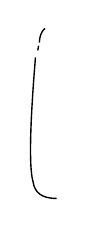
\begin{tikzpicture}[x=1cm,y=1cm,baseline] \draw[line width=.5pt] (.15,2.2) .. controls (.1,2.16) and (.08,2.08) .. (.08,2.02); \draw[line width=.5pt] (.07,1.98) -- (.06,1.92); \draw[line width=.5pt] (.03,1.83) .. controls (-.03,1.1) and (-.06,.45) .. (0,.25) .. controls (.02,.12) and (.1,.04) .. (.3,.04); \end{tikzpicture}}
équivalence près, on peut supposer qu'il s'agit de vrais groupes dans
(Cat), \deleted{resp. de vraie commutativité.}

\margin{\handwritten{8}}
